
\documentclass[../../layout.tex]{subfiles}

\begin{document}
\chapter{Fundamentação teórica}
\hspace*{3em}O estudo, entendimento e compreensão dos conceitos abordados nesse projeto são de extrema importância para sua compreensão.

\section{Internet das Coisas}
\hspace*{3em}Com o desenvolvimento e demanda massiva de um mundo mais tecnológico, muitos conceitos sobre tecnologia foram surgindo e moldando a sociedade \acite{iot}. Uma dessas tecnologias em que fazemos uso é a \emph{IoT}, na qual podemos brevemente resumir em um sistema de equipamentos, dispositivos, máquinas, objetos ou pessoas que possam se comunicar entre si, com identificações únicas, capazes de transferir dados através de conexões ou redes sem necessitar interação humana ou de um humano com uma máquina \cite{iot}. Exemplos reais são carros capazes de enviar sinais ao celular do motorista quando a pressão dos pneus está baixa ou monitoramento de um implante de coração pela central de um hospital, em que esses dados possam ser endereçados utilizando um protocolo de internet (IP). O objetivo principal da \emph{IoT} é fazer com que essas comunicações sejam mais eficientes, rápidas, seguras e até influenciar tomadas de decisões. Um sistema em que utiliza o conceito de internet das coisas pode ser organizado em:

\begin{enumerate}[label=\alph*)]
\itemsep0em
\item coleta de dados gerados por sensores, aparelhos ou máquinas;
\item consolidação e envio dos dados através de uma conexão;
\item análise dos dados para realizar ações ou tomada de decisões.
\end{enumerate}

\hspace*{3em} Na figura \ref{fig:iotsystem} de um sistema \emph{IoT} se comunicando, onde uma camada coleta os dados por meio de um dispositivo (sensor, antena ou microcontrolador), esses dados são transmitidos por um \emph{hub} (dispositivo intermediário, ou responsável pela transmissão dos dados), por fim são analisados e as ações são executadas.

\begin{figure}[H]
\centering
\caption{Exemplo de um sistema \emph{IoT}}
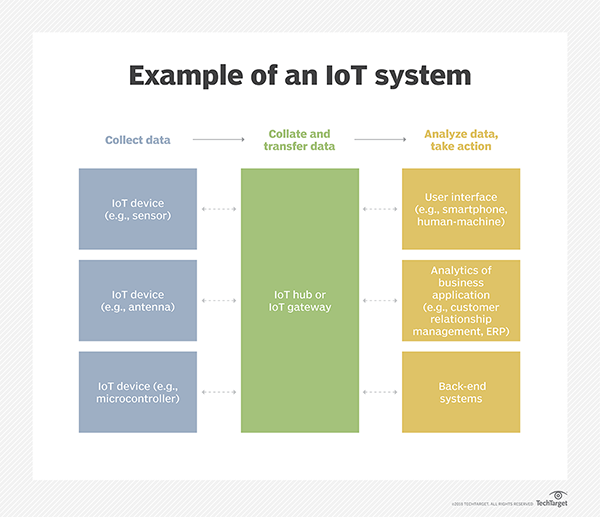
\includegraphics[width=0.7\textwidth]{assets/static/img/iot_system.jpg}
\label{fig:iotsystem}

\begin{minipage}{0.5\textwidth}
\raggedright \footnotesize Fonte: Retirado de \cite{iotsystem} 
\end{minipage}
\end{figure}

\subsection{Evolução da Internet das Coisas}
\hspace*{3em}Na década de 90 a internet foi capaz de facilitar muitos negócios, porém era muito impactada ainda pela velocidade de conexão e dificuldade de acesso \cite{iothouse}. Nos anos 2000 a conectivade com a internet se tornou mais popular ao ponto de muitas aplicações se tornarem dependentes dela. Atualmente a dependência da internet aumentou porém, ainda é necessária a interação do ser humano e/ou de outras máquinas para que as ações sejam executadas. É nesse contexto que se insere a \emph{IoT},por exemplo, o acesso à uma página da internet para pesquisas ou realização vendas online podem ser executados de maneira dinâmica e automatizada. \par
Essa ideia é mais comum ainda nos dias atuais, pois temos várias "coisas" dentro de residências que se comunicam de maneira automatizada e muitas vezes podem  ser controladas via um aplicativo de celular, um navegador de internet no computador ou até mesmo uma central eletrônica. Na Figura \ref{fig:iothou} temos um exemplo de uma casa inteligente conectada.

\begin{figure}[H]
\centering
\caption{Exemplo de uma casa conectada por um sistema \emph{IoT}}
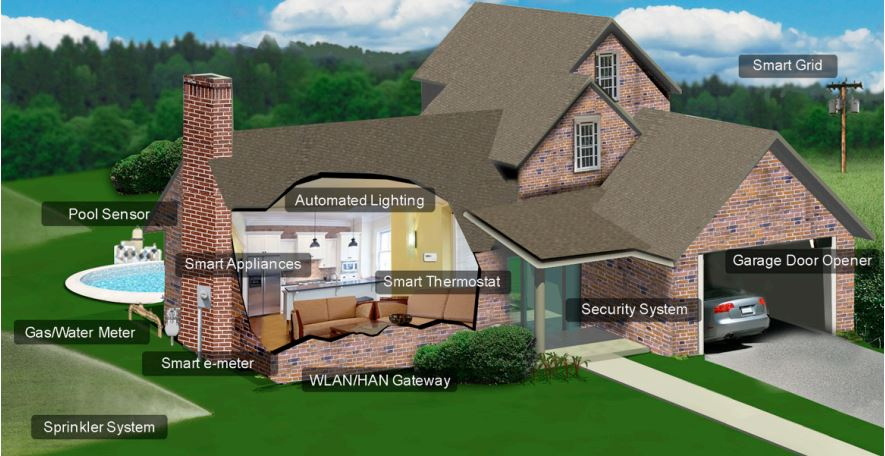
\includegraphics[width=0.7\textwidth]{assets/static/img/iothouse.jpg}
\label{fig:iothou}

\begin{minipage}{0.5\textwidth}
\raggedright \footnotesize Fonte: Retirado de \cite{iothouse} 
\end{minipage}
\end{figure}

\subsection{Indústria 4.0}

\hspace*{3em}Com a evolução da era digital, muitos setores foram impctados para ter seu melhor desempenho e crescimento. A transformação digitalização da manufatura que ocorreu durante vários anos, desde a primeira revolução industrial em que eram utilizadas máquinas à vapor, a segunda na qual utilizava eletricidade como revolução, a terceira em que se fez o uso de computadores e máquinas eletrônicas até a quarta na qual tende a emergir a terceira revolução com computadores mais avançados capazes de automatizar uma linha completa com sistemas inteligentes e interligados em que o ponto principal é o tratamento de dados sendo alimentados e gerados por esses computadores \cite{ind4}.A figura \ref{fig:ind} demonstra essa evolução.

\begin{figure}[H]
\centering
\caption{Revoluções Industriais}
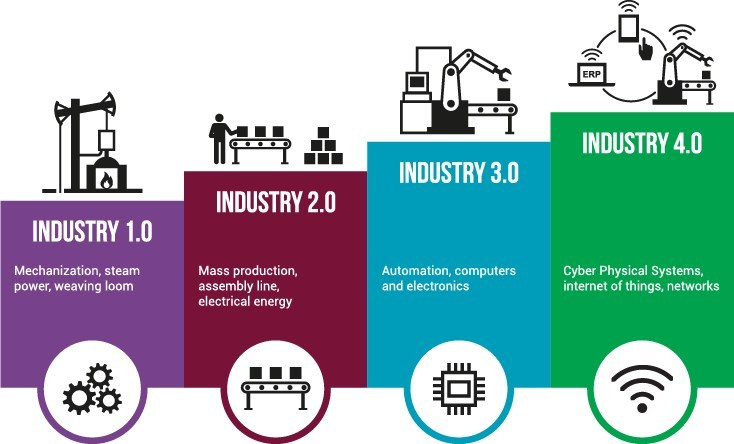
\includegraphics[width=0.5\textwidth]{assets/static/img/ind4.jpg}
\label{fig:ind}

\begin{minipage}{0.7\textwidth}
\raggedright \footnotesize Fonte: Retirado de \cite{ind4} 
\end{minipage}
\end{figure}


\hspace*{3em}Muitos modelos de tecnologia podem ser abordados para alavancar a Indústria 4.0. Exemplos desses modelos são:
\begin{enumerate}[label=\alph*)]
\itemsep0em
    \item combinações de sistemas ciberfísicos, computacionais colaborativos que controlam entidades ou equipamentos físicos \cite{cyberphysic};
    \item internet das coisas;
    \item aprendizado de máquina (\emph{Machine Learning}).
\end{enumerate}

\hspace*{3em}Esses exemplos citados são meios utilizados para trazer valores dentro da indústria por exemplo, para que sejam feitas análises através de inúmeros dados gerados e coletados sobre performance, manutenção, rendimento e defeitos com o objetivo de identificar oportunidades, otimizar logística e a sua cadeia de gestão (\emph{Supply Chain}). Robôs inteligentes para facilitar o processo ou logística de linhas, carros autônomos para automatizar o processo e segurança de locomoção, máquinas autônomas que possam ser totalmente independentes da interação humana para executar sua função e até impressão 3D são alguns dos muitos sucessos da aplicação da Indústria 4.0 no mercado atual. Apesar de parecer que estamos vivenciando essa revolução hoje em dia, estima-se que essa revolução irá permanecer em evolução durante 30 anos em que aos poucos as empresas vão adotando em seus processos.

\section{Modelo utilizado para aplicação}
\hspace*{3em}Para o desenvolvimento da aplicação utilizamos o modelo cliente servidor em três camadas. Esse modelo permite a modularização da aplicação em: camada de interface com usuário, também conhecida como \emph{front-end}, camada lógica onde estão inseridas as regras de negócios, também conhecido como \emph{back-end} e a camada de dados  onde se realiza a comunicação com o banco de dados. Essa arquitetura permite um desacoplamento de código que viabiliza a atualização das partes de forma independente da tecnologia \cite{3layers}
\section{Conceito do REST API}
\hspace*{3em}REST (Transferência representacional de estado) API (Interface de programação de aplicação) analisando os conceitos isolados.\par
API é uma interface de comunicação  disponível por software com regras estabelecidas para que haja o entendimento de ambas as partes. Esse conceito é aplicado para criar uma camada de abstração, no qual para utilizar os recursos de um determinado software é apenas necessário o entendimento da interface disponibilizada por um software, eliminando a  necessidade do entendimento total do software, além de viabilizar o conceito de modularização de arquitetura de software. \cite{16} \par 
REST é um modelo de arquitetura criado para suprir conceitos de qualidade e funcionalidade, em princípio para sistemas distribuídos. Acabou sendo utilizada largamente em servidores WEB, tanto para a maneira em que a arquitetura define um conjunto de restrições para uma arquitetura estilo REST, quanto para padrões uniformes para interfaces, sem conservação de estado e separação total do cliente e servidor. Com isso, permitindo a interoperabilidade entre sistemas. Quando um servidor WEB segue esses conceitos, pode ser denominado de REST FULL.\par

Portanto uma REST API é uma interface que aplica os conceito REST para sua implementação\cite{19}. Quando o protocolo HTTP é utilizado, o URI (Identificador de recursos uniformes) se torna uma representação dos dados e os métodos HTTP são utilizados para manipular esses dados \cite{16}, com os métodos:

\begin{enumerate}[label=\alph*)]
\itemsep0em
    \item GET para recuperar os dados;
    \item POST para criar novos dados;
    \item PUT para atualizar os dados;
    \item DELETE para apagar os dados.
\end{enumerate}

\section{Backend}
\subsection{Conceito de Back-end}
\hspace*{3em}Uma aplicação WEB em geral é dividida  em duas principais partes, a camada do \emph{front-end} que é responsável pela interação com o usuário de forma gráfica e o \emph{back-end} é responsável por entregar toda a lógica necessária para o \emph{front-end}, geralmente o \emph{back-end} é dividido em três elementos responsáveis por implementar a lógica do negócio \cite{16}:

\begin{enumerate}[label=\alph*)]
\itemsep0em
    \item aplicação;
    \item banco de dados;
    \item servidor.
\end{enumerate}

\subsection{Linguagem Back-end}
\hspace*{3em}A linguagem mais utilizada para programar dispositivos IoT é a linguagem C por ser mais otimizada para essa finalidade, mas por ser uma linguagem de baixo nível, exige uma extensa dedicação de tempo e torna-se moroso para soluções mais complexas. Para contornar essas deficiências, a linguagem Elixir pode ser uma ótima alternativa, por ser uma linguagem de alto nível que não compromete tanto a performance do sistema.\par
A linguagem Erlang/Elixir é uma linguagem funcional desenvolvida para atingir alta performance e confiabilidade. Foi desenvolvida para aplicações voltadas para telecomunicações que exigem, baixa tolerância de falhas, distribuida e \emph{real-time} (tempo de execução). Por isso conta com um conjunto bibliotecas para desenvolvimento de sistemas de alta confiabilidade conhecida como OTP.\par
Elixir foi desenvolvida para ser executada na VM (máquina virtual) do Erlang nomeada como BEAM. A linguagem Elixir é relativamente nova, mas já existem diversas aplicações que a utilizam e inclusive existem recursos para dispositivo embarcado como o \emph{framework} Nerves \cite{ElixirorIoT} e para implementação de aplicações WEB como o \emph{framework} Phoenix.

\subsection{Nerves}
\hspace*{3em}Nerves é um \emph{framework} para desenvolvimento de projetos embarcados, baseado em Linux que apenas executa a VM BEAM, portanto, proporcionando a utilização da linguagem Elixir para o desenvolvimento das aplicações,  desfrutando do potencial da linguagem para implementação de projetos embarcados. Além disso, este \emph{framework} proporciona diversas vantagens em relação ao processo tradicional de programação de embarcados \cite{nerves}, como:

\begin{enumerate}[label=\alph*)]
\itemsep0em
    \item permitir a fácil portabilidade para diferentes HW (hardware) embarcados e com uma vasta abrangência para diferentes HW embarcados;
    \item fácil manutenção e atualização de firmware por viabilizar a atualizações via OTA (atualização sobre o ar);
    \item dispensa o processo tradicional de dispor do acesso físico, à flash do dispositivo para o armazenamento do firmware;
    \item recursos para facilitar e agilizar o desenvolvimento de firmware;
    \item vasta biblioteca para manipulação dos sistemas embarcados.
\end{enumerate}

\subsection{Phoenix}

\hspace*{3em}Phoenix é um \emph{framework} desenvolvido em Elixir para implementação de aplicações WEB, que usa todo o potencial da linguagem Elixir, com isso desfrutando da concorrência fornecida pela VM BEAM, com baixa tolerância a falha e baixa latência.  Além de aumentar o desempenho do desenvolvimento de uma aplicação WEB também conta com diversos recurso que são disponibilizados de forma modular \cite{phoenix}. Na figura \ref{fig:diagrama_sw} temos um diagrama detalhado da arquitetura utilizada no projeto.

\begin{figure}[H]
\centering
\caption{Diagrama simplificado da arquitetura do software}
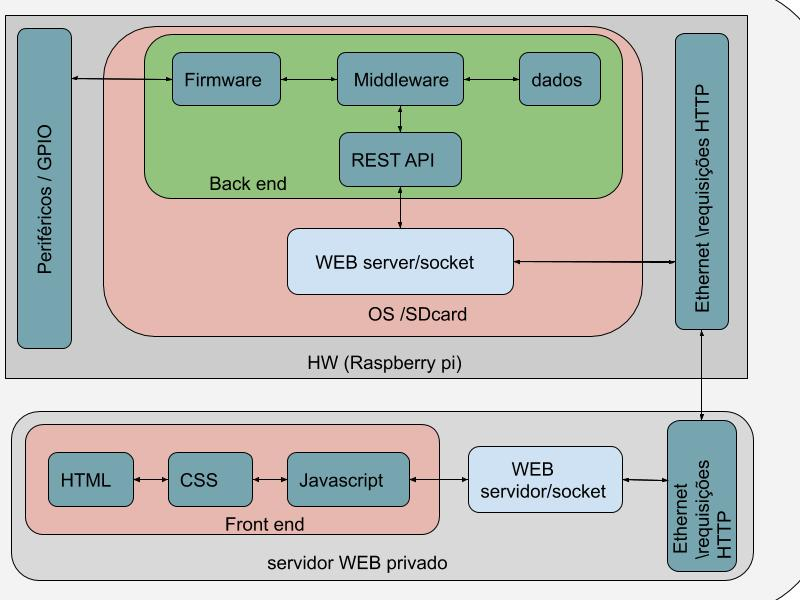
\includegraphics[width=0.8\textwidth]{assets/static/img/diagrama_tcc.jpg}
\label{fig:diagrama_sw}
\end{figure}

\section{Frontend}
\subsection{Conceito de Front-end}
\hspace*{3em}Em uma aplicação WEB a camada de \emph{front-end} é responsável por realizar a interação com usuário, e  também é conhecida por \emph{client-side} (lado do cliente), pois todos os recursos desenvolvidos são executados em um \emph{web browser} (navegador web) alocado em um computador pessoal. Para que essa interface com o usuário seja criada sob demanda, é necessário um fluxo de comunicação entre o \emph{browser} e o servidor. Em geral, o \emph{browser} solicita a partir do protocolo HTTP uma requisição para o servidor onde está hospedado todas as informações visuais necessárias, o backend do servidor recebe essa requisição, então realiza as alterações necessárias no servidor e retorna com o conteúdo solicitado. O conteúdo é composto por códigos HTML, CSS e JavaScript, o \emph{browser} recebe esse pacote e renderiza de forma visual a informação solicitada. Essas são as três tecnologias essenciais para a construção de uma interface visual WEB.\cite{frontend}

\subsection{Mobile Front-end}
\hspace*{3em}Por  muitos anos o \emph{front-end} teve como objetivo o \emph{browser} para PC, portanto, os \emph{layouts} eram desenvolvidos para telas dentro das dimensões padrões dos computadores. Entretanto, com o advento dos dispositivos móveis, foram necessárias adaptações à tecnologia que apesar de muito prematura, já demonstrava o seu potencial. Criaram-se então os conceitos de \emph{design} responsivo e \emph{mobile-first} (movél primeiro) que tem como objetivo criar interfaces que podem ser adaptadas para quaisquer que sejam as dimensões das telas, desde um computador até dispositivos como \emph{smartwatch}.\par
Com a tendência de acesso à páginas WEB a partir de quaisquer dispositivos móveis, houve um realce no potencial da tecnologia IoT, viabilizando o controle de qualquer dispositivo a partir de até mesmo um pequeno \emph{smartwatch} em qualquer lugar do mundo.\cite{mobilefrontend}

\subsection{Hyper Text Markup Language (HTML)}
\hspace*{3em}É uma linguagem de marcação padrão para o desenvolvimento WEB, que descreve a estrutura de uma \emph{webpage} de forma semântica, por isso é considerada uma linguagem de marcação ao invés de uma linguagem de programação. Essa descrição é renderizada pelo navegador WEB em uma forma gráfica.\cite{frontend}

\subsection{Cascading Style Sheets (CSS)}
\hspace*{3em}Também é considerada uma linguagem de marcação, porém com o objetivo de criar uma folha de estilo para páginas WEB. É muito utilizada para modificar a estrutura de uma página WEB escrita em HTML. O CSS demonstra um aspecto mais moderno com muito mais recursos visuais e de design para as aplicações WEB. Isso se dá pois o CSS permite alterações no \emph{layout} geral do texto e da página, além de permitir mais agilidade nas aplicações, por diminuir o tamanho dos arquivos em relação ao HTML.\cite{frontend}

\subsection{Javascript}
\hspace*{3em}Javascript é uma linguagem de programação interpretada, multi-paradigma, dinâmica e sem tipos, voltada para desenvolvimento WEB. Em comparação às linguagens HTML e CSS, que são voltadas para a criação de elementos estáticos na aplicação WEB, o Javascript permite o desenvolvimento de aplicações mais complexas, trazendo mais dinâmica e versatilidade para as aplicações WEB.\cite{frontend}

\section{Arquivo JSON e XML}
\hspace*{3em}Para padronizar a transmissão de informações atavés de aplicações e dispositivos diferentes, foram criados vários formatos de texto para sua formatação ideal à aplicação, desenvolvedores e ao próprio usuário. Dessa forma a escolha deve ser analisada para melhor praticidade, desempenho e segurança. O formato JSON (\textit{JavaScript Object Notation}) é utilizado em aplicações compactas, de padrão aberto e de fácil compreensão , sendo muito prática para serem visualizadas de forma geral e escritas ao mesmo tempo, ao contrário de formatações como o XML (\textit{Extensible Markup Language}), o JSON é uma formatação totalmente independente que surgiu do JavaScript, porém usa convensões familiares de outras linguagens da família C (C, C++, C\#), Python, Pearl, o que a torna muito prática para formatação em várias plataformas. A seguir, exemplos da formatação em XML e JSON:

\begin{enumerate}[label=\alph*)]
\itemsep0em
  \item XML:
    \begin{minted}[xleftmargin=\parindent,tabsize=2,breaklines]{xml}
<?xml version="1.0" encoding="UTF-8"?>
<cardapio>
<comida>
    <nome>Hot Dog</nome>
    <preco>R$ 8,99</preco>
    <descricao>
   	Pão com salsicha completo (acompanha batata palha, ketchup e maionese)
   	</descricao>
    <calorias>650</calorias>
</comida>
<comida>
    <nome>Hamburguer</nome>
    <preco>R$ 10,99</preco>
    <descricao>
    Pão com 1 fatia de hambúrguer, 3 fatias de tomate, salada, ketchup e 1 fatia de queijo
    </descricao>
    <calorias>950</calorias>
</comida>
</cardapio>
    \end{minted}
  
  \item JSON:
    \begin{minted}[xleftmargin=\parindent,tabsize=2,breaklines]{js}
[
   {
      "nome": "Hot Dog",
      "preco": "R$ 8,99",
      "descricao": "Pão com salsicha completo (acompanha batata palha, ketchup e maionese)",
      "calorias": "650"
   },
   {
      "nome": "Hamburguer",
      "preco": "R$ 10,99",
      "descricao": "Pão com 1 fatia de hambúrguer, 3 fatias de tomate, salada, ketchup e 1 fatia de queijo",
      "calorias": "950"
   }
]
    \end{minted}
\end{enumerate}

O formato JSON, como mencionado, tem um visual mais limpo, com uma leitura mais simples do arquivo e maior velocidade na manipulação e transmissão dos dados.

\section{Segurança em software}
\hspace*{3em}Com o crescimento da tecnologia \emph{IoT}, nasceram novos problemas de segurança, uma vez que existe uma grande diversidade e quantidade de objetos conectados na rede. O principal problema se dá pela falta de cuidado no design de software o que abre caminho para que \emph{malwares} e \emph{backdoors} se instalem. Além disso, a dificuldade de identificar os objetos na rede e gerar métodos de autenticação seguros (métodos tradicionais não são aplicáveis devido a heterogeneidade dos objetos) são importantes problemas a serem solucionados. Outro obstáculo está em manter a privacidade dos dispositivos \emph{IoT}. Durante o uso da tecnologia, dados do comportamento e da rotina diária são coletados a fim de melhorar os serviços e a experiência pessoal de cada usuário. Entretanto, as informações coletadas descrevem o usuário detalhadamente, assim é necessário cautela quanto à exposição desses dados, para evitar o uso indevido de informações pessoais. 
É importante ainda ter em mente, que alguns dispositivos possuem capacidade de computacional limitada e restrições de consumo elétricos por terem  baterias limitadas, portanto, não suportam  sistemas complexos de criptografia por exigirem poder computacional elevado e consequentemente o aumentando do consumo elétrico. Algoritmos mais simplificados de criptografia são mais adequados para dispositivos com restrição de recursos. Uma segunda solução é ocultar alguns dados, porém isso ainda é um obstáculo uma vez que os objetos conectados precisam ter acesso a tais informações. \cite{seguranca}

\section{Protocolos de comunicação}
\end{document}
\hspace*{3em}Com a demanda do uso de tecnologias relacionadas à área de Internet das Coisas, várias camadas de comunicação e estruturas se adaptam para maior praticidade do uso de dispositivos diversos, que por sua grande maioria se tratam de microcontroladores e sensores, na qual estão conectados entre si, seja por LAN (\emph{Local Area Network}) ou WiFi (\emph{Wireless Fidelity}). Para que essa comunicação seja eficaz e segura, foram padronizados protocolos de comunicação que são vastamente utilizados no período atual por várias empresas.

\subsection{i2c}
\hspace*{3em}O I2C é um protocolo de comunicação em que o dado é transferido \emph{bit} a \emph{bit} através de uma única conexão de uma maneira síncrona, fazendo com que a saída desse sinal seja baseada no \emph{clock} (período de oscilação) enviado do \emph{Master} (Mestre) ao \emph{Slave} (Escravo), onde esse \emph{clock} é apenas dependente do Master. Esse método de comunicação necessita apenas de 2 conexões, o SDA (\emph{Serial Data Access}) e o SCL (\emph{Serial Clock Access}).

\begin{figure}[H]
\centering
\caption{Protocolo I2C}
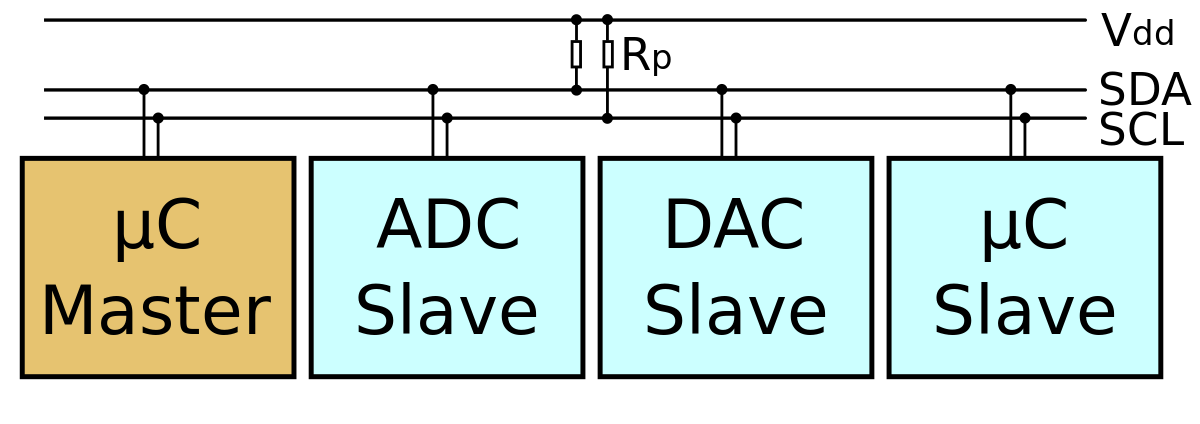
\includegraphics[width=0.5\textwidth]{assets/static/img/i2c.jpg}
\label{fig:i2c}

\begin{minipage}{0.5\textwidth}
\raggedright \footnotesize Fonte: Retirado de \acite{i2c} 
\end{minipage}
\end{figure}

\hspace*{3em}Com a comunicação via I2C, os dados são quebrados em pequenos pacotes em que formam esse padrão. Esses pacotes contém informações do endereço do \emph{Slave}, \emph{bits} de condição de início e fim da menssagem transmitida, o dado a ser transmitido e um sinal de \emph{feedback} chamado de positivo ACK (\emph{Acknowledge bit}) quando a mensagem é entregue ao escravo, ou negativo NACK (\emph{No-acknowledge bit}) quando a mensagem não é entregue ao escravo, de acordo com a figura \ref{fig:i2cstructure}.

\begin{figure}[H]
\centering
\caption{pacote i2c}
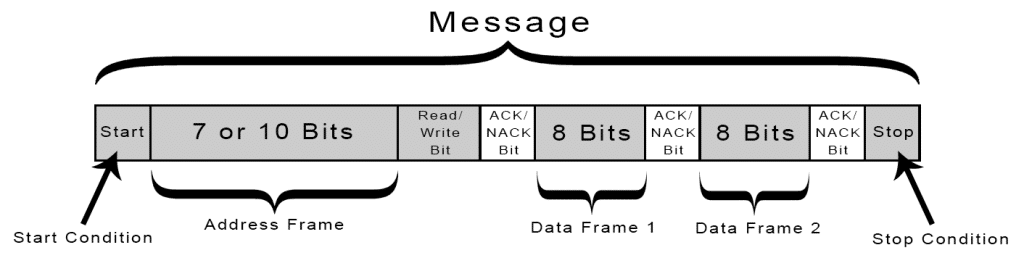
\includegraphics[width=0.5\textwidth]{assets/static/img/i2c_structure.jpg}
\label{fig:i2cstructure}

\begin{minipage}{0.5\textwidth}
\raggedright \footnotesize Fonte: Retirado de \cite{i2c_structure} 
\end{minipage}
\end{figure}

\subsection{UART}
\hspace*{3em}A comunicação UART (\emph{Universal Asynchronous Receiver-Transmitter}) é um dispositivo presente dentro de um microcontrolador em que seu objetivo é controlar a entrada e saída de dados através de sequências de 8 \emph{bits}. Atualmente é o método mais comum para comunicação serial \emph{full-duplex} \cite{uart} A comunicação UART não se refere apenas à um protocolo, mas um conjuto completo de circuitos integrados. Os dispositivos UART possuem duas conexões, uma para transmitir dados (TX) e outra para receber os dados (RX), de uma maneira totalmente assíncrona ao \emph{clock}. Da mesma forma que citamos do I2C, o UART também utiliza \emph{bits} para identificação do início e fim do pacote enviado ou recebido. Importante citar que todos os dispositivos no circuito devem ter o mesmo \emph{baud rate} (taxa de transmissão) como padronização.
\end{document}
